% Created 2023-03-03 Fri 15:44
% Intended LaTeX compiler: pdflatex
\documentclass[presentation, aspectratio=1610]{beamer}
\usepackage[utf8]{inputenc}
\usepackage[T1]{fontenc}
\usepackage{graphicx}
\usepackage{longtable}
\usepackage{wrapfig}
\usepackage{rotating}
\usepackage[normalem]{ulem}
\usepackage{amsmath}
\usepackage{amssymb}
\usepackage{capt-of}
\usepackage{hyperref}
\usetheme[progressbar=foot]{metropolis}
\usepackage{caption}
\captionsetup[figure]{labelformat=empty}
\usetheme{metropolis}
\usecolortheme{}
\usefonttheme{}
\useinnertheme{}
\useoutertheme{}
\author{Andrew Jensen}
\date{March 9, 2023}
\title{Joint Track Machine Learning}
\hypersetup{
 pdfauthor={Andrew Jensen},
 pdftitle={Joint Track Machine Learning},
 pdfkeywords={},
 pdfsubject={},
 pdfcreator={Emacs 28.1 (Org mode 9.6)}, 
 pdflang={English}}
\usepackage{biblatex}
\addbibresource{/home/andrew/repo/lit-review/src/myBib.bib}
\addbibresource{~/org/biblio.bib}
\begin{document}

\maketitle
\begin{frame}{Outline}
\tableofcontents
\end{frame}


\section{Introduction}
\label{sec:orgb2902ec}
\begin{frame}[label={sec:orgafd70f2}]{Acknowledgments}
I would like to thank the McJunkin Family Charitable Foundation for their generous grant that supports this work.
\end{frame}
\section{Motivation}
\label{sec:org001d7c7}
\begin{frame}[label={sec:org955693d}]{The Problem}
\begin{columns}
\begin{column}{0.5\columnwidth}
\begin{itemize}
\item 20\% of patients receiving TKA are dissatisfied.
\begin{itemize}
\item Instability, pain, unnatural \autocites{bakerRolePainFunction2007}[][]{bournePatientSatisfactionTotal2010}[][]{scottPredictingDissatisfactionFollowing2010}.
\end{itemize}
\item No reliable method of clinically assessing and quantifying joint dynamics.
\begin{itemize}
\item Too much human supervision, too time consuming
\end{itemize}
\end{itemize}
\end{column}
\begin{column}{0.5\columnwidth}
\begin{center}
\includegraphics[width=\textwidth]{/home/andrew/repo/lit-review/figures/raster/Physical_Examination_of_the_knee.jpg}
\end{center}
\end{column}
\end{columns}
\end{frame}
\begin{frame}[label={sec:orgdb30d3b}]{Our Proposition}
\begin{columns}
\begin{column}{0.5\columnwidth}
Orthopaedic surgeons and clinicians would readily adopt a practical and inexpensive technology that allows them to measure a patient's knee kinematics during activities of daily living.
\end{column}
\begin{column}{0.55\columnwidth}
\begin{center}
\includegraphics[width=2in]{/home/andrew/repo/lit-review/figures/raster/dynamic-knee-prescription.png}
\end{center}
\end{column}
\end{columns}
\end{frame}
\begin{frame}[label={sec:org716c681}]{Constraints}
\begin{columns}
\begin{column}{0.45\columnwidth}
\begin{itemize}
\item It must fit within a standard clinical workflow
\item The technology must utilize equipment commonly found in hospitals
\item There must not be significant human supervision nor interaction to generate an examination report.
\end{itemize}
\end{column}
\begin{column}{0.55\columnwidth}
\begin{center}
\includegraphics[width=\textwidth]{/home/andrew/repo/lit-review/figures/raster/c-arm-fluoro-machine.jpg}
\end{center}
\end{column}
\end{columns}
\end{frame}
\section{Background}
\label{sec:org9e35d80}
\begin{frame}[label={sec:orgecc7171}]{Rigid Body Transformations}
\begin{block}{Translation}
\begin{equation*}
  \begin{aligned}
  \begin{pmatrix}
    v_{x}' \\ v_{y}'
  \end{pmatrix} &=
  \begin{pmatrix}
    v_{x} \\ v_{y}
  \end{pmatrix} +
  \begin{pmatrix}
    t_{x} \\ t_{y}
  \end{pmatrix} \\
                & \rightarrow \\
    \begin{pmatrix}
      v_{x}' \\ v_{y}' \\ 1
    \end{pmatrix} &=
                    \begin{pmatrix}
                      1 & 0 & t_{x} \\ 0 & 1 & t_{y} \\ 0 & 0 & 1
                    \end{pmatrix}
                                                                \begin{pmatrix}
                                                                  v_{x} \\ v_{y} \\  1
                                                                \end{pmatrix}
\end{aligned}
\end{equation*}
\end{block}
\end{frame}

\begin{frame}[label={sec:orgdebe1b0}]{Rigid Body Transformations}
\begin{block}{Rotations}
\begin{equation*}
  \begin{aligned}
    R_{x} & =
            \begin{pmatrix}
              1 & 0 & 0 \\
              0 & c_{x} & -s_{x}\\
              0 & s_{x} & c_{x}
            \end{pmatrix} \\
    R_{y} &=
            \begin{pmatrix}
              s_{y} & 0 & c_{y}\\
              0 & 1 & 0 \\
              c_{y} & 0 & -s_{y}
            \end{pmatrix} \\
    R_{z} &=
            \begin{pmatrix}
              c_{z} & -s_{z} & 0 \\
              s_{z} & c_{z} & 0 \\
              0 & 0 & 1
            \end{pmatrix}
  \end{aligned}
\end{equation*}
\end{block}
\end{frame}

\begin{frame}[label={sec:org32bb84e}]{Rigid Body Transformations}
\begin{block}{Homogeneous Transformation Matrices}
\begin{equation*}
  \begin{aligned}
  \tilde{\vec{v'}} &=
  \begin{pmatrix}
    & \mathbf{R}_{3 \times 3} & & \vec{t}_{3 \times 1} \\
    0 & 0 & 0 & 1
  \end{pmatrix}\tilde{\vec{v}} \\
    &= T^{A}_{B} \tilde{\vec{v}}
  \end{aligned}
\end{equation*}

Now we have a notation that allows us to describe arbitrary movement between reference frames.
\end{block}
\end{frame}
\begin{frame}[label={sec:org1eab471}]{Projective Geometry}
\begin{columns}
\begin{column}{0.5\columnwidth}
\begin{equation*}
  \begin{pmatrix}
    x_{s} \\ y_{s} \\ z_{s} \\ 1
  \end{pmatrix}_{i} = T^{cam}_{scene} \mathbf{\tilde{p}^{obj}_{i}}
\end{equation*}

\begin{equation*}
  \begin{pmatrix}
    \tilde{x}_{img} \\ \tilde{y}_{img} \\ \tilde{z}
  \end{pmatrix} =
  \begin{pmatrix}
    f& 0 & 0 \\ 0 & f & 0 \\ 0 & 0 & 1
  \end{pmatrix} \vec{x}_{s}
\end{equation*}

Where
\begin{equation*}
  \begin{aligned}
    x_{img} &= \frac{\tilde{x_{img}}}{\tilde{z}} = \frac{f}{z_{s}}x_{s} \\
    y_{img} &= \frac{\tilde{y_{img}}}{\tilde{z}} = \frac{f}{z_{s}}y_{s}
  \end{aligned}
\end{equation*}

{\tiny Note: We are still in the camera's reference frame}
\end{column}

\begin{column}{0.6\columnwidth}
\begin{center}
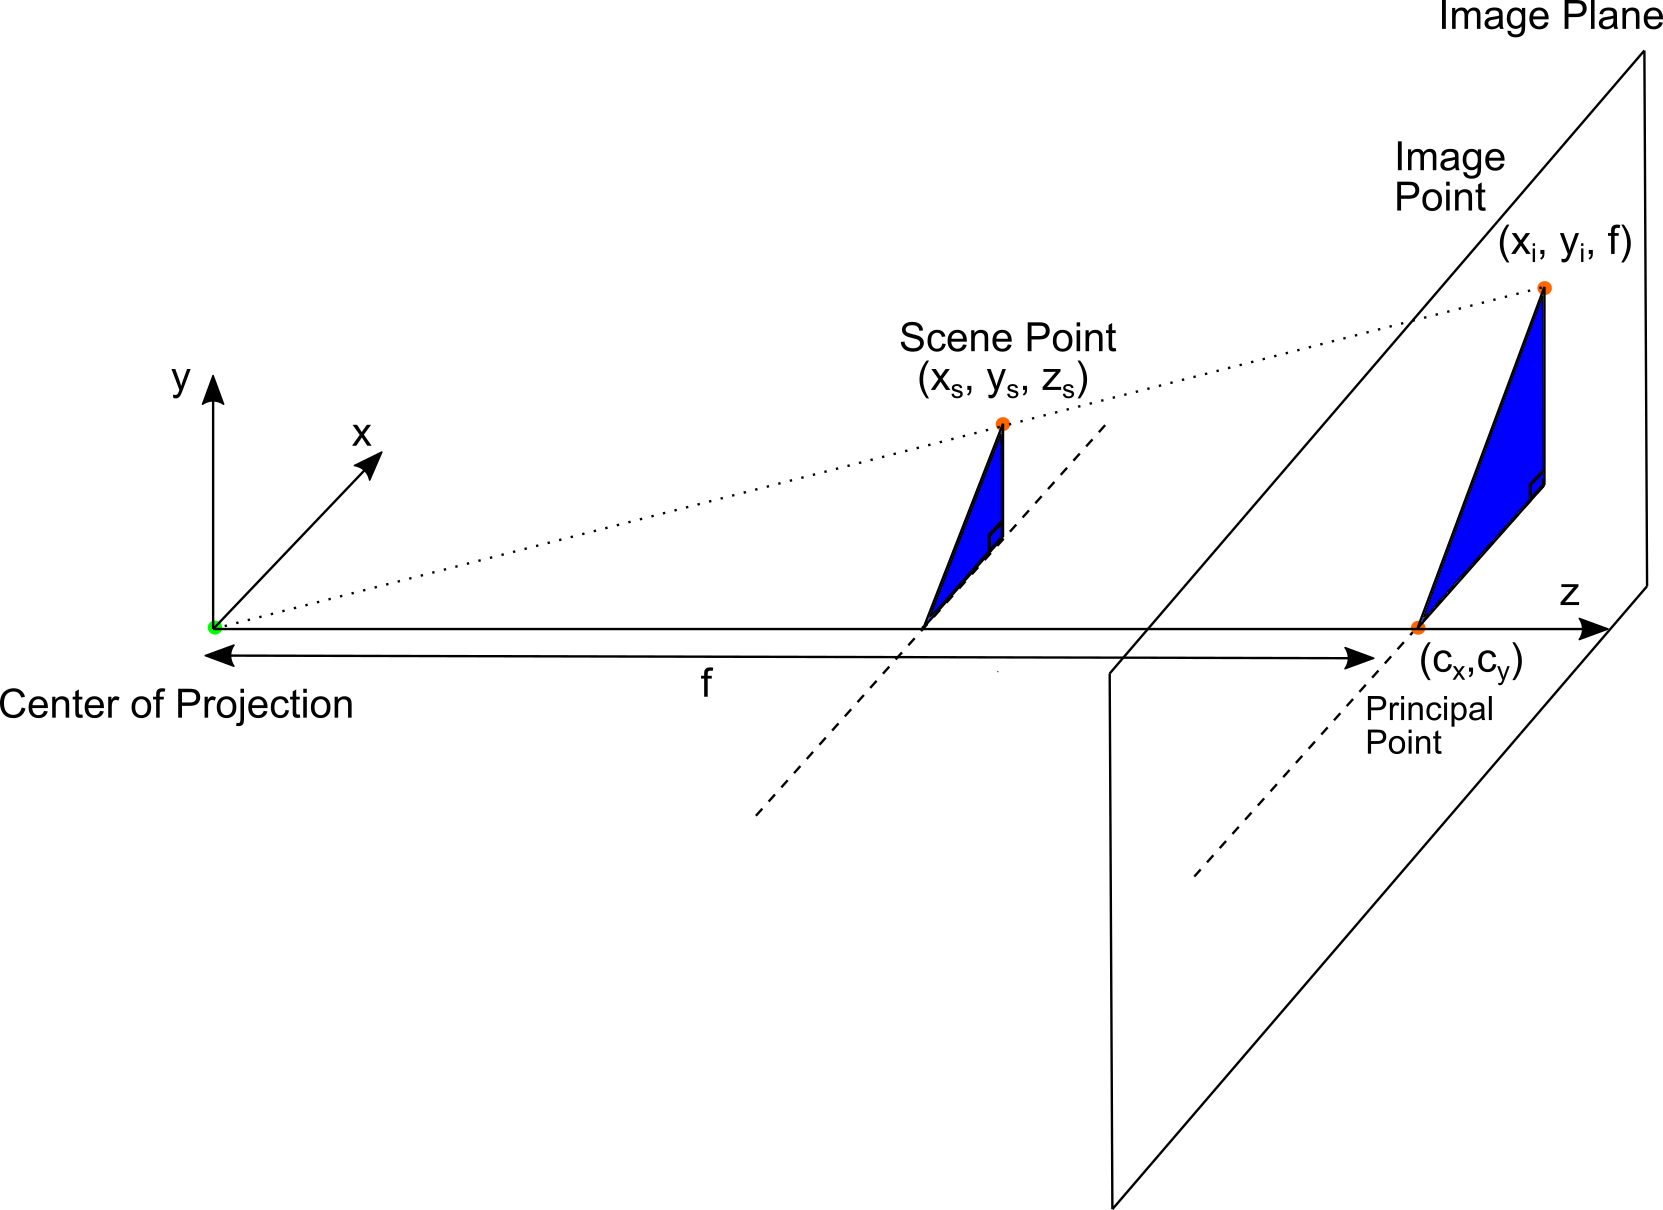
\includegraphics[width=.9\linewidth]{/home/andrew/repo/lit-review/figures/raster/perspective-projection.png}
\end{center}
\end{column}
\end{columns}
\end{frame}
\begin{frame}[label={sec:orgaeb4544}]{Pixel Coordinates}
Convert camera coordinates into image coordinates.
\begin{equation*}
  \begin{aligned}
    p_{x} = k_{x}x_{img} + c_{x} \\
    p_{y} = k_{y}y_{img} + c_{y}
  \end{aligned}
\end{equation*}
Where
\begin{equation*}
  \begin{aligned}
    k &\equiv \text{ Pixel Spacing }\\
    c &\equiv \text{ Image Focal Point }
  \end{aligned}
\end{equation*}
\end{frame}

\begin{frame}[label={sec:orgbf5c759}]{Model-Image Registration}
\begin{columns}
\begin{column}{0.5\columnwidth}
If we know the projective parameters of the fluoroscopy machine, can we tinker with \(T^{cam}_{implant}\) so that our virtual projection matches the fluoroscopic image?
\end{column}
\begin{column}{0.6\columnwidth}
\begin{figure}[htbp]
\centering
\includegraphics[width=2.5in]{/home/andrew/repo/lit-review/figures/raster/mahfouz-perspective-projection.png}
\caption{From \autocite{mahfouzRobustMethodRegistration2003}}
\end{figure}
\end{column}
\end{columns}
\end{frame}
\section{Historical Methods}
\label{sec:orge6e841b}
\begin{frame}[label={sec:org7427e88}]{Overview}
Many different approaches have attempted to solve the model-image registration problem.
\begin{itemize}
\item Pre-computed projections
\item Skin-mounted motion Capture
\item Biplane Imaging
\item Iterative Projections
\item Model-based Roentgen Stereophotogrammetry
\end{itemize}
\end{frame}
\begin{frame}[label={sec:orgfedbfbf}]{Pre-Computed Projections}
\begin{columns}
\begin{column}{0.5\columnwidth}
\begin{itemize}
\item Saving space and memory by pre-computing as much as possible.
\item Pre-computed distance maps \autocites{zuffiModelbasedMethodReconstruction1999}[][]{lavalleeRecoveringPositionOrientation1995}.
\item Pre-computed shape libraries \autocite{banksAccurateMeasurementThreedimensional1996}
\end{itemize}
\end{column}
\begin{column}{0.6\columnwidth}
\begin{figure}[htbp]
\centering
\includegraphics[width=1.75in]{/home/andrew/repo/lit-review/figures/raster/lavallee-distance-maps.png}
\caption{From \autocite{lavalleeRecoveringPositionOrientation1995}}
\end{figure}
\vspace{-0.25in}
\begin{figure}[htbp]
\centering
\includegraphics[width=1.75in]{/home/andrew/repo/lit-review/figures/raster/banks-nfd-library.png}
\caption{From \autocite{banksAccurateMeasurementThreedimensional1996}}
\end{figure}
\end{column}
\end{columns}
\end{frame}
\begin{frame}[label={sec:org5d209cb}]{Limitations of Pre-Computed Projections}
\begin{itemize}
\item Requires an accurate contour from the input image in order to perform calculations.
\begin{itemize}
\item Human supervision vs. inaccuracy.
\end{itemize}
\end{itemize}
\end{frame}

\begin{frame}[label={sec:org39df3e1}]{Motion Capture (MoCap)}
\begin{columns}
\begin{column}{0.5\columnwidth}
\begin{itemize}
\item Can measure motion of MoCap beads very accurately.
\item Skin-mounted \autocites{gaoInvestigationSoftTissue2008}[][]{kuoInfluenceSoftTissue2011}[][]{linEffectsSoftTissue2016}.
\item Bone pins \autocite{lafortuneThreedimensionalKinematicsHuman1992} (any volunteers?).
\end{itemize}
\end{column}

\begin{column}{0.6\columnwidth}
\begin{figure}[htbp]
\centering
\includegraphics[width=2.5in]{/home/andrew/repo/lit-review/figures/raster/gao-skin-mocap.png}
\caption{From \autocite{gaoInvestigationSoftTissue2008}}
\end{figure}
\vspace{-0.25in}
\begin{figure}[htbp]
\centering
\includegraphics[width=2.5in]{/home/andrew/repo/lit-review/figures/raster/lafortune-bone-mocap.png}
\caption{From \autocite{lafortuneThreedimensionalKinematicsHuman1992}}
\end{figure}
\end{column}
\end{columns}
\end{frame}
\begin{frame}[label={sec:org1db63e1}]{Limitations of Motion Capture}
Skin Mounted
\begin{itemize}
\item Doesn't accurately describe underlying skeletal motion with clinical accuracy \autocites{gaoInvestigationSoftTissue2008}[][]{kuoInfluenceSoftTissue2011}[][]{linEffectsSoftTissue2016}.
\end{itemize}
Bone Pins
\begin{itemize}
\item Bone Pins
\item Need I say more?
\end{itemize}
\end{frame}
\begin{frame}[label={sec:org16c5e1a}]{Biplane Imaging}
\begin{columns}
\begin{column}{0.5\columnwidth}
\begin{itemize}
\item Utilizes multiple cameras to resolve 3D position and orientation\autocites{ivesterReconfigurableHighSpeedStereoRadiography2015}[][]{burtonAutomaticTrackingHealthy2021}.
\begin{itemize}
\item Highly accurate.
\item Gold Standard.
\end{itemize}
\end{itemize}
\end{column}
\begin{column}{0.6\columnwidth}
\begin{figure}[htbp]
\centering
\includegraphics[width=1.75in]{/home/andrew/repo/lit-review/figures/raster/ivester-stereo-fluoromachine.png}
\caption{Both from \autocite{ivesterReconfigurableHighSpeedStereoRadiography2015}}
\end{figure}
\vspace{-0.25in}
\begin{figure}[htbp]
\centering
\includegraphics[width=1.75in]{/home/andrew/repo/lit-review/figures/raster/ivester-stereo-projection.png}
\end{figure}
\end{column}
\end{columns}
\end{frame}
\begin{frame}[label={sec:orgc2e4696}]{Limitations of Biplane Imaging}
\begin{itemize}
\item Not many hospitals have biplane fluoroscopy setups.
\item Clinically impractical
\end{itemize}
\end{frame}

\begin{frame}[label={sec:org9ef8460}]{Iterative Projections}
\begin{columns}
\begin{column}{0.54\columnwidth}
\begin{itemize}
\item Take advantage of modern computational graphics pipelines to quickly perform projection matching.
\begin{itemize}
\item Image/Intensity similarity metrics \autocite{mahfouzRobustMethodRegistration2003}
\item Feature/Contour similarity metrics \autocite{floodAutomatedRegistration3D2018}
\end{itemize}
\end{itemize}
\end{column}
\begin{column}{0.6\columnwidth}
\begin{figure}[htbp]
\centering
\includegraphics[width=2in]{/home/andrew/repo/lit-review/figures/raster/mahfouz-perspective-projection.png}
\caption{From \autocite{mahfouzRobustMethodRegistration2003}}
\end{figure}
\begin{figure}[htbp]
\centering
\includegraphics[width=2in]{/home/andrew/repo/lit-review/figures/raster/flood-dilated-contour.png}
\caption{From \autocite{floodAutomatedRegistration3D2018}}
\end{figure}
\end{column}
\end{columns}
\end{frame}
\begin{frame}[label={sec:org27f211b}]{Limitations of (historic) Iterative Projection Methods}
\begin{itemize}
\item Requires human supervision for:
\begin{itemize}
\item Pose initialization
\item Escaping local minima
\item Implant detection
\end{itemize}
\item Chaotic and Noisy objective function
\end{itemize}
\end{frame}

\begin{frame}[label={sec:orgbe42b15}]{Model-based Roentgen Stereophotogrammetry (MBRSA)}
\begin{columns}
\begin{column}{0.5\columnwidth}
\begin{itemize}
\item Uses implanted tantalum beads for motion tracking \autocites{vroomanFastAccurateAutomated1998}[][]{selvikRoentgenStereophotogrammetryMethod1989}
\item Extremely accurate \autocites{kapteinEvaluationThreePose2004}[][]{saariKneeKinematicsMedial2005}
\item Gold standard Measurement \autocite{brobergValidationMachineLearning2023}
\end{itemize}
\end{column}

\begin{column}{0.6\columnwidth}
\begin{figure}[htbp]
\centering
\includegraphics[width=3in]{/home/andrew/repo/lit-review/figures/raster/vrooman-mbrsa.png}
\caption{From \autocite{vroomanFastAccurateAutomated1998}}
\end{figure}
\end{column}
\end{columns}
\end{frame}
\begin{frame}[label={sec:orgc46e55f}]{Limitations of MBRSA}
\begin{itemize}
\item Involves additional surgical procedures for inserting tantalum beads
\item Human supervision
\item Typically requires bi-plane imaging.
\end{itemize}
\end{frame}

\begin{frame}[label={sec:org13c5a9f}]{Aims page}
Aims
\end{frame}
\begin{frame}[label={sec:org1c23b49}]{Aims}
\begin{columns}
\begin{column}{0.3\columnwidth}
\begin{block}{Aims 1/2}
Joint Track Machine Learning and Overcoming Single-Plane Limitations
\end{block}
\end{column}
\begin{column}{0.3\columnwidth}
\begin{block}{Aim 3/4}
Pilot Trials and Standardized Kinematics Exam
\end{block}
\end{column}
\begin{column}{0.3\columnwidth}
\begin{block}{Aim 5}
Joint Track Auto Toolkit
\end{block}
\end{column}
\end{columns}
\end{frame}

\section{Aim 1 - Joint Track Machine Learning}
\label{sec:org07b9677}
\begin{frame}[label={sec:orgc9a3a7c}]{Goal}
Demonstrate the feasibility of a fully autonomous, model-image registration pipeline.
\end{frame}
\begin{frame}[label={sec:orge9959e5}]{Method}
\begin{itemize}
\item Three-tiered approach
\begin{itemize}
\item Convolutional Neural networks (CNN) for autonomous implant detection
\item Normalized Fourier Descriptor shape libraries
\item Robust contour-based global optimization scheme
\end{itemize}
\end{itemize}
\begin{center}
\includegraphics[width=.9\linewidth]{/home/andrew/repo/lit-review/figures/raster/pipeline-nocite.png}
\end{center}
\end{frame}
\begin{frame}[label={sec:org19adf55}]{Autonomous Implant Detection Using Convolutional Neural Networks}
\begin{columns}
\begin{column}{0.5\columnwidth}
\begin{itemize}
\item 2 CNNs
\begin{itemize}
\item Femoral and Tibial implants
\end{itemize}
\item High Resolution Network \autocite{wangDeepHighResolutionRepresentation2020}
\end{itemize}
\end{column}
\begin{column}{0.5\columnwidth}
\begin{center}
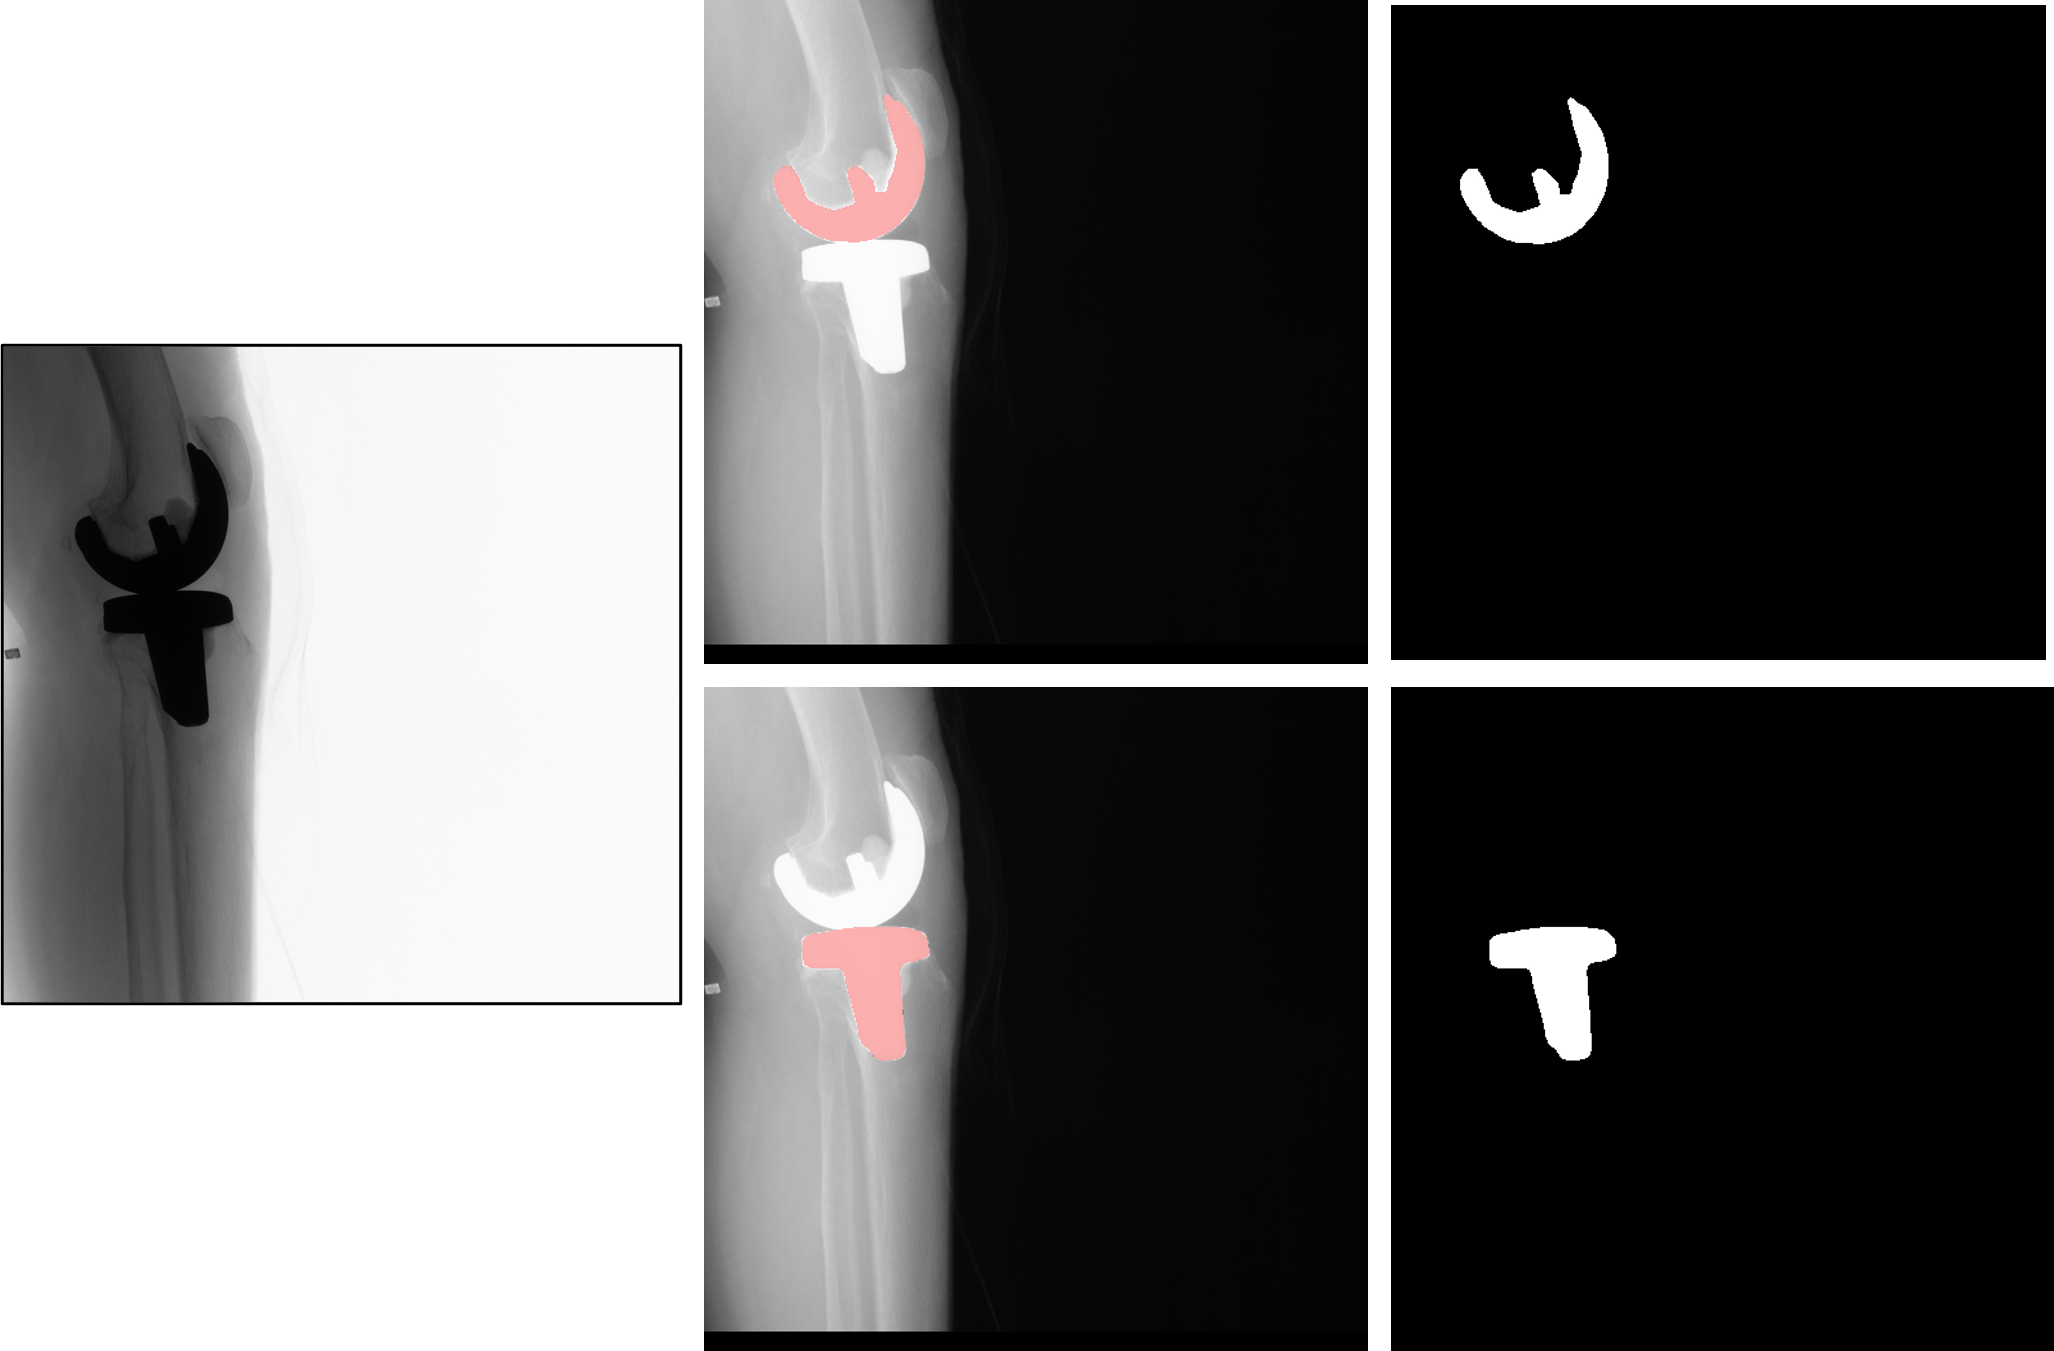
\includegraphics[width=\columnwidth]{/home/andrew/repo/lit-review/figures/raster/jtml-segmentation.png}
\end{center}
\end{column}
\end{columns}
\end{frame}
\begin{frame}[label={sec:org4e28048}]{Neural Network Data}
\begin{columns}
\begin{column}{0.5\columnwidth}
\begin{itemize}
\item \textasciitilde{}8000 images
\begin{itemize}
\item 7 TKA kinematics studies
\item PUT DATA INFO HERE!!!!!
\end{itemize}
\end{itemize}
\end{column}

\begin{column}{0.6\columnwidth}
\begin{center}
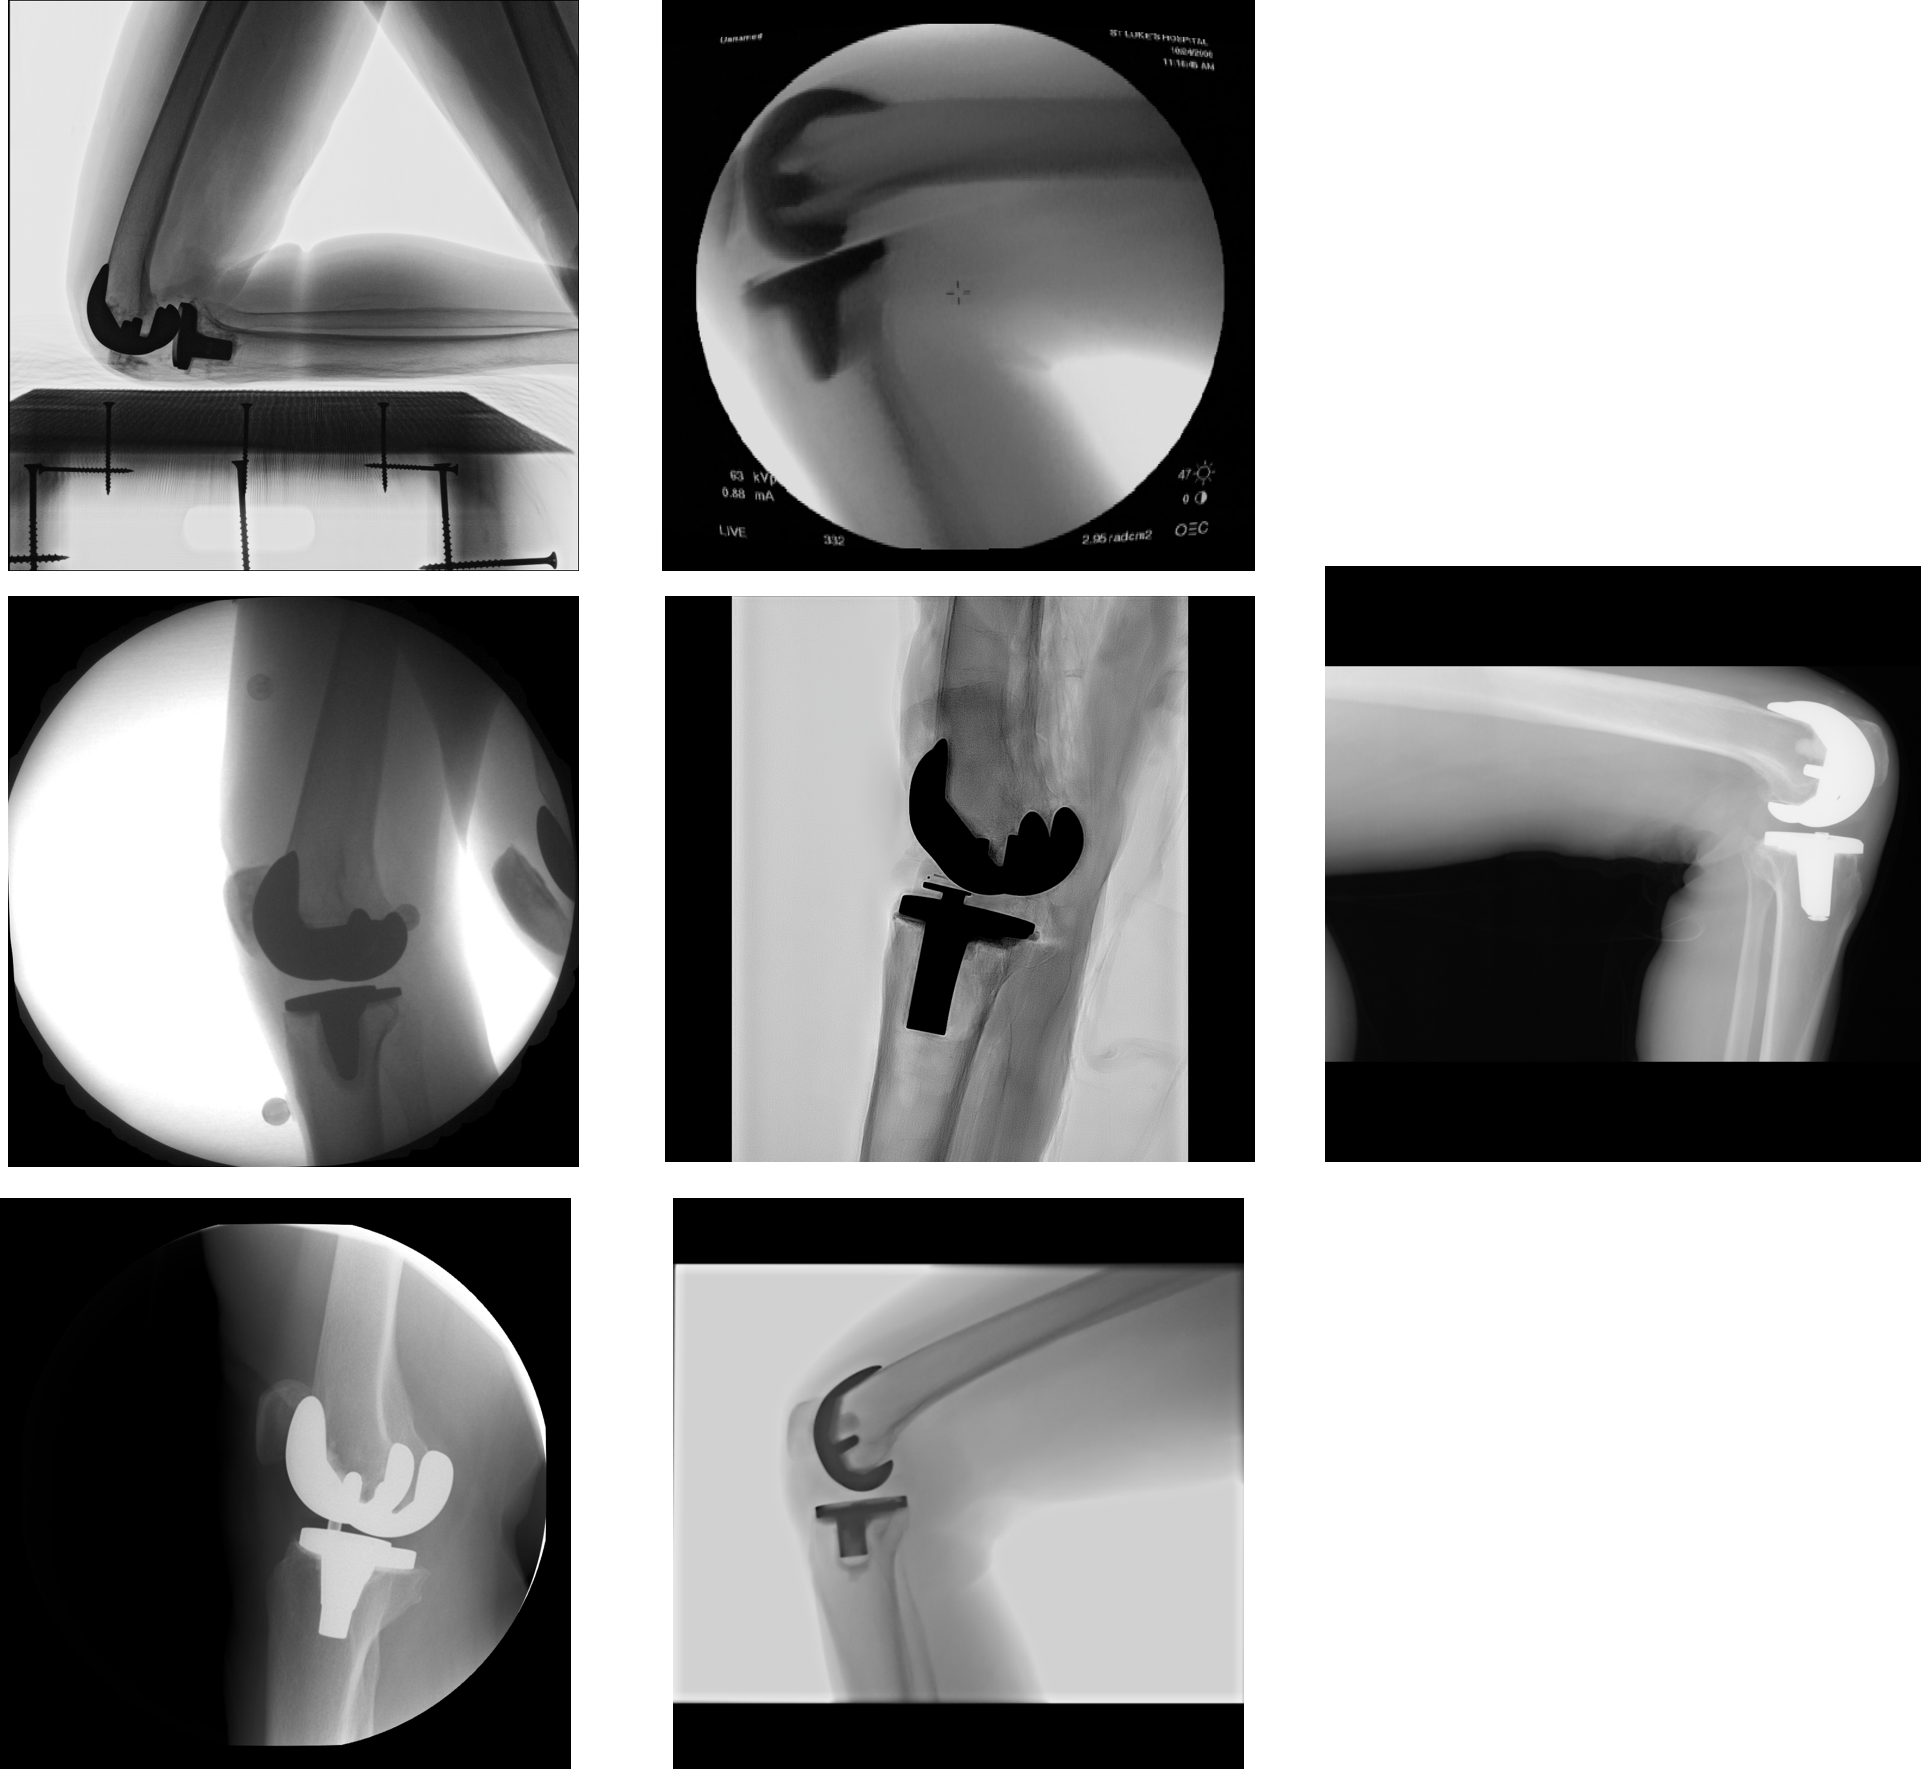
\includegraphics[height=3in]{/home/andrew/repo/lit-review/figures/raster/jtml-data.png}
\end{center}
\end{column}
\end{columns}
\end{frame}
\begin{frame}[label={sec:org63f306b}]{Neural Network Robustness}
\begin{itemize}
\item Additional augmentations introduced during training \autocite{buslaevAlbumentationsFastFlexible2020}.
\end{itemize}
\begin{center}
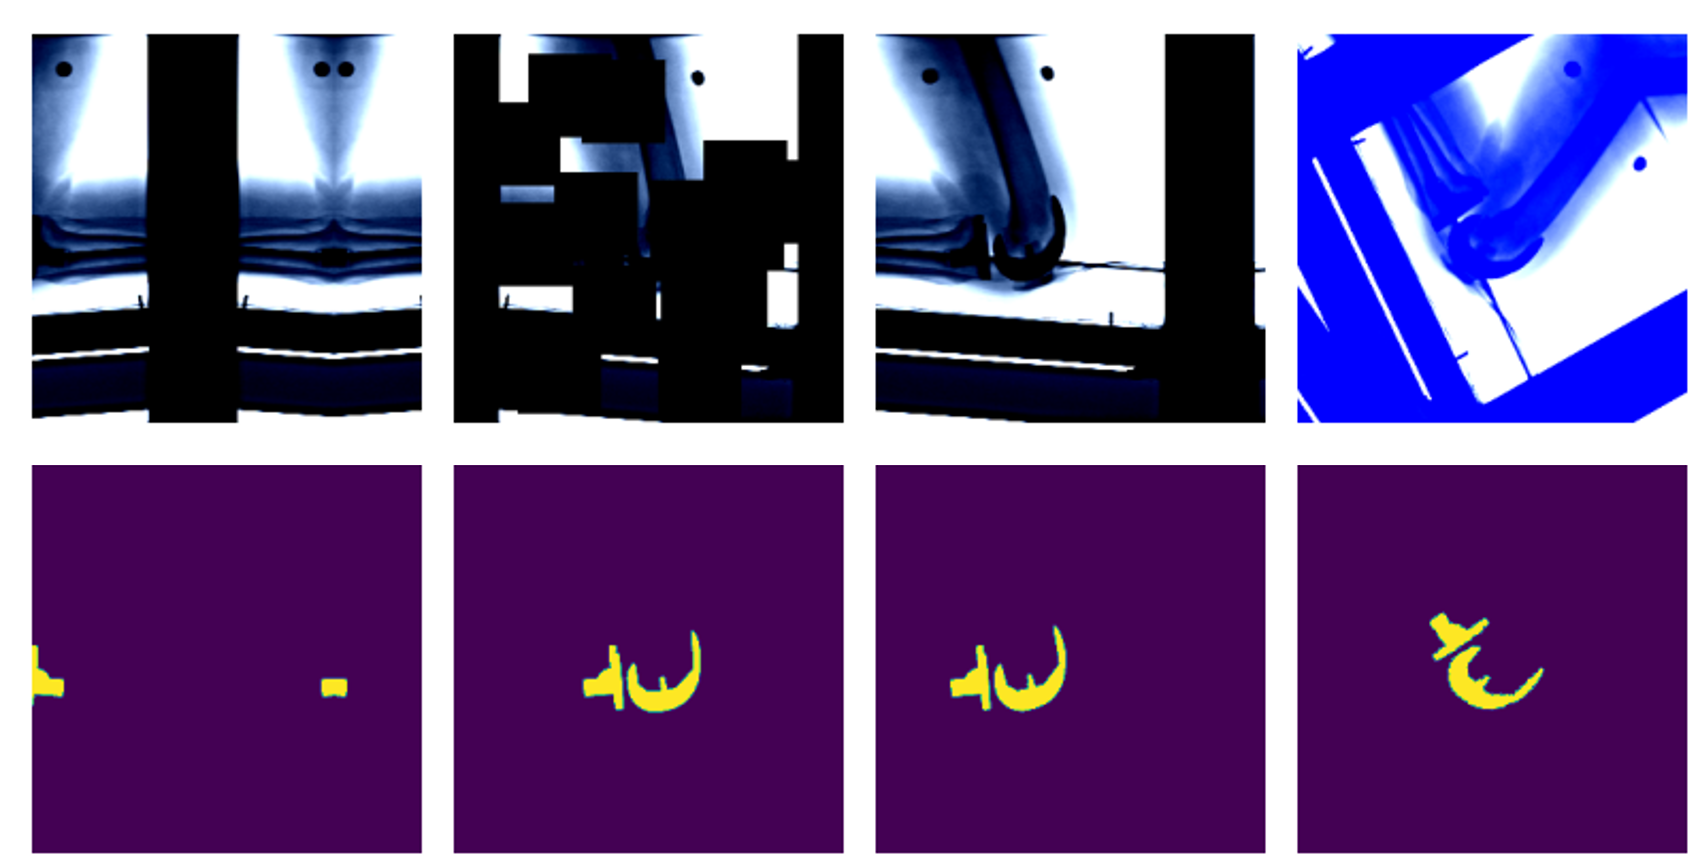
\includegraphics[width=.9\linewidth]{/home/andrew/repo/lit-review/figures/raster/augmentations.png}
\end{center}
\end{frame}
\begin{frame}[label={sec:org1cf6e5c}]{Normalized Fourier Descriptor Shape Libraries}
\begin{columns}
\begin{column}{0.37\columnwidth}
\begin{itemize}
\item Pose initialization using segmentation output.
\item \(\pm 30^{\circ}\) library span at \(3^{\circ}\) increments.
\end{itemize}
\end{column}

\begin{column}{0.7\columnwidth}
\begin{center}
\includegraphics[width=2in]{/home/andrew/repo/lit-review/figures/raster/banks-nfd-library.png}
\end{center}
\begin{center}
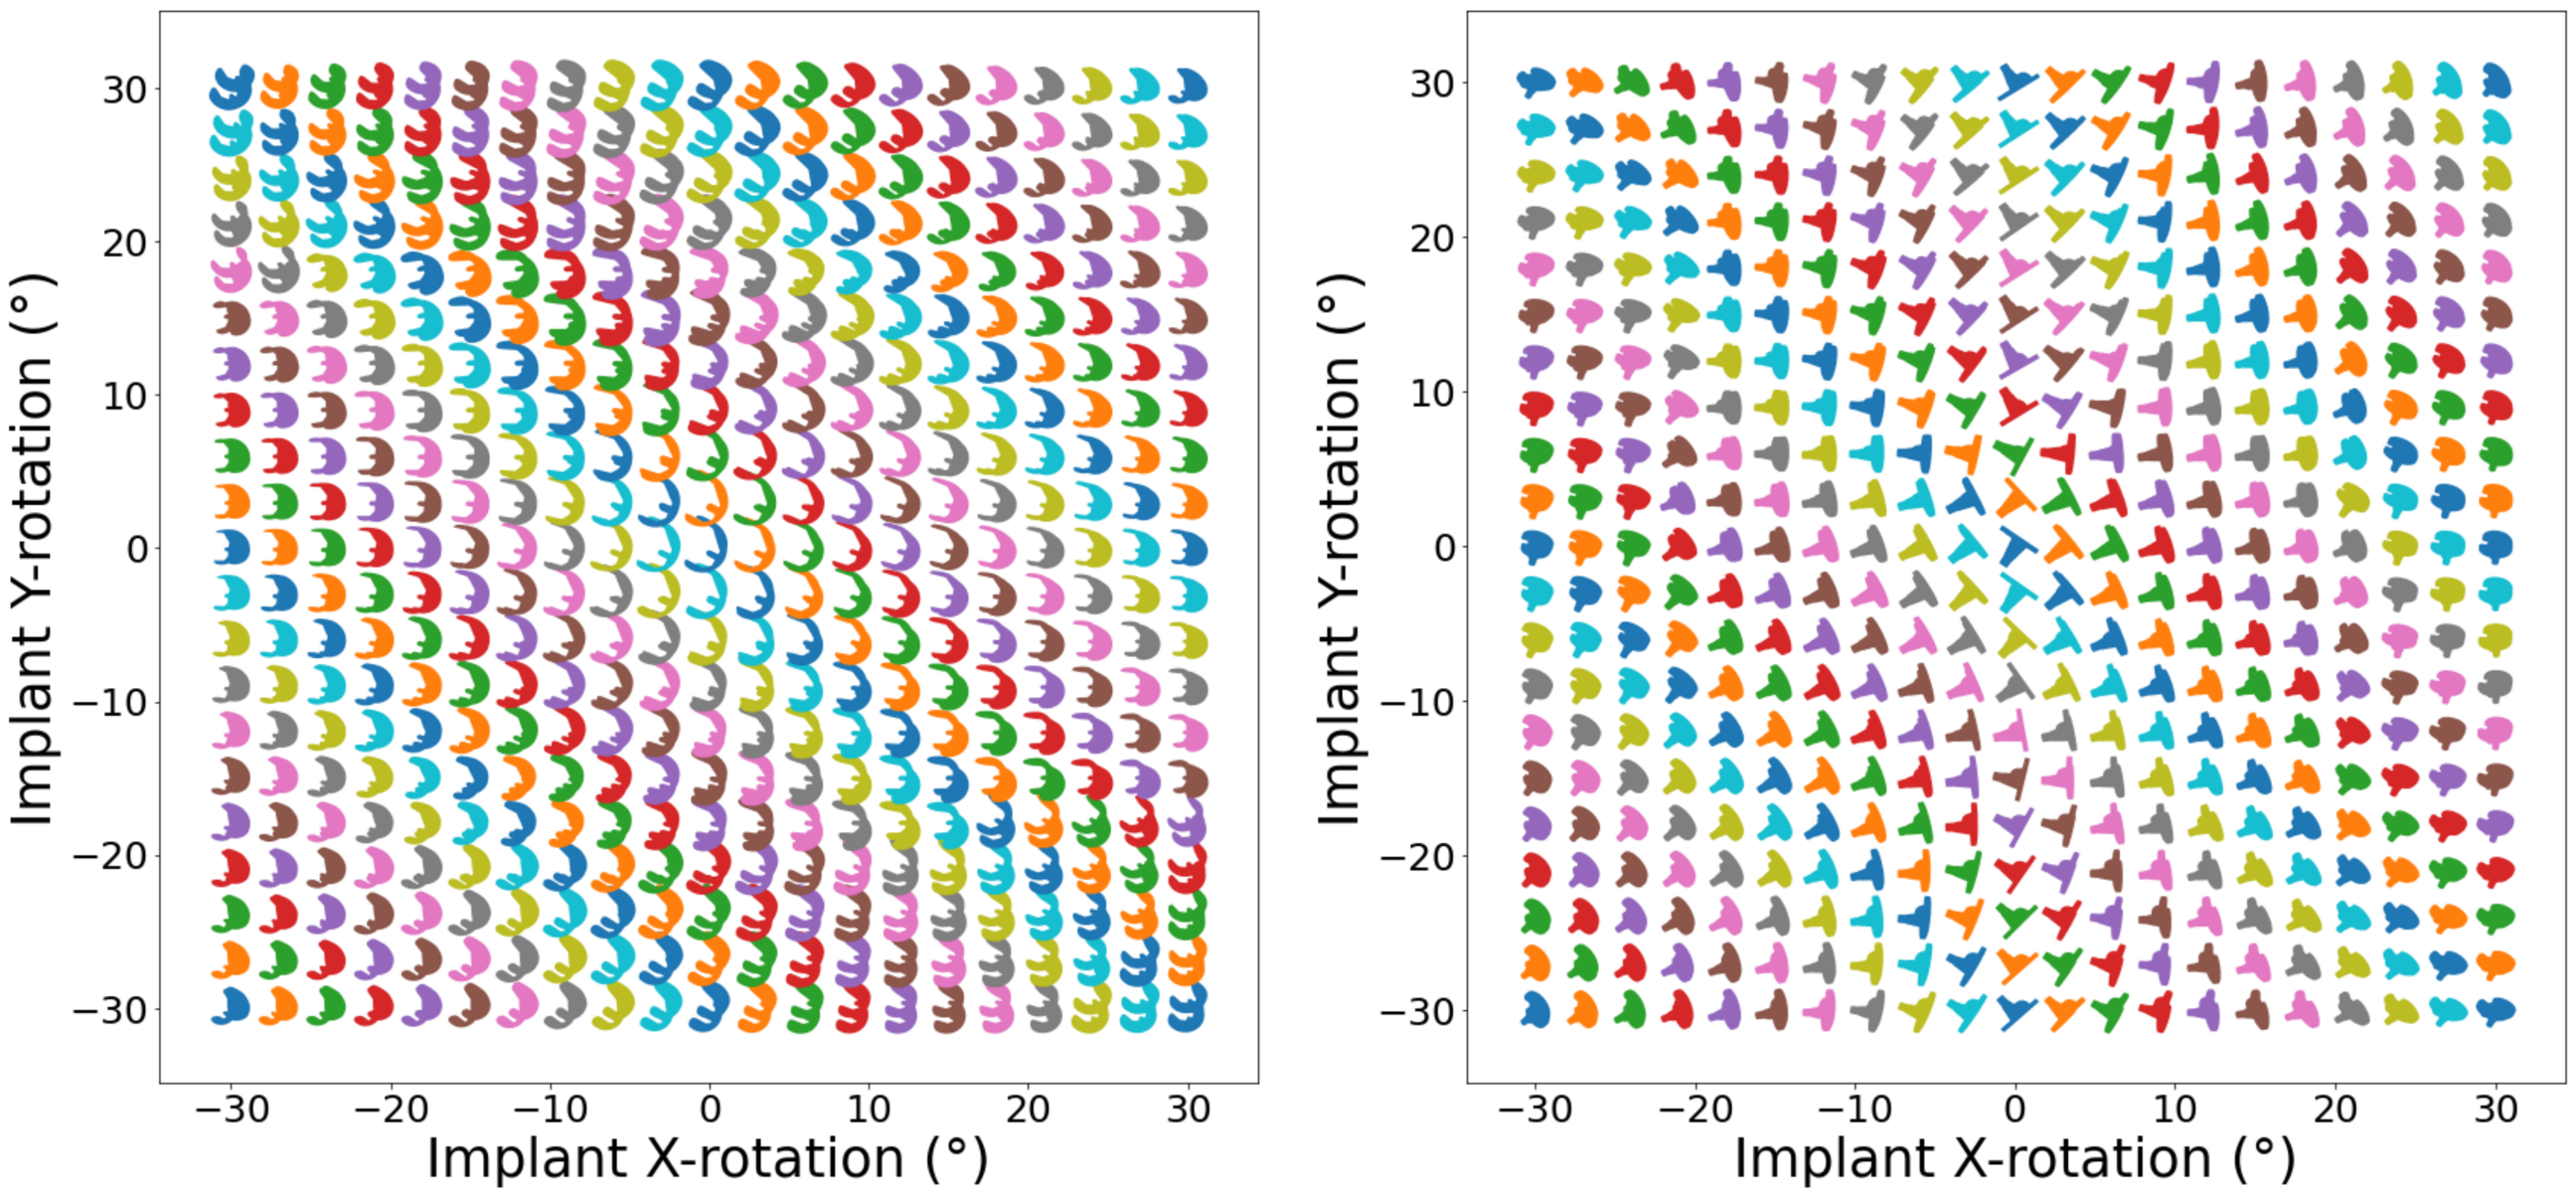
\includegraphics[width=3.25in]{/home/andrew/repo/lit-review/figures/raster/jtml-nfd.png}
\end{center}
\end{column}
\end{columns}
\end{frame}
\section{References}
\label{sec:orgadde541}
\begin{frame}[label={sec:org83615c1},fragile, allowframebreaks, label=]{References}
\AtNextBibliography{\tiny}
\printbibliography
\end{frame}
\end{document}